\chapter{Análise Bibliográfica sobre o uso de transformers no processamento de linguagem natural, por Daniel Rodrigues Cardoso}

\section{Planejamento do estudo}
O processamento de linguagem natural é uma das áreas que mais tem movimentado pesquisas no ramo da inteligencia artificial e com o passar dos anos novas técnicas estão surgindo. Uma técnica que tem ganhado bastante notoriedade se da por meio do uso de transformers e que sera o elemento de estudo desta pesquisa.

Esta pesquisa foi concebida com o intuito de sanar as seguintes questões:
\begin{itemize}
    \item Como o uso de transformers para processamento de linguagem natural evoluiu durante o tempo?
    
    \item De que forma o uso de transformers impactou os estudos em processamento de linguagem natural?
    
    \item Quais os autores mais relevantes?
\end{itemize}



\subsection{Limitações}Durante a produção deste trabalho a maior limitação foi o tempo disponível para o desenvolvimento do mesmo. foram empregadas cerca de 9 horas, tempo este que foi divido entre aprender a utilizar as ferramentas necessárias (R Studio e bibliometrix) e na coleta e análise dos dados.

\section{Coleta de dados}
A coleta de dados foi realizada utilizando a ferramenta de busca Web Of Science no dia 9 de fevereiro de 2022, acessado por meio do Portal de Periódicos da Capes.

\subsection{Query de Busca}
Para a busca, foi usada a \query\ abaixo:
\begin{verbatim}
(transformer*) 
and (Natural Language Processing or nlp)
\end{verbatim}
\subsubsection{Explicação para os termos de busca usados}
O foco deste trabalho era obter resultados que tratassem do uso de transformers no processamento de linguagem natural, desta forma a palavra chave transformer* foi adotada, para refinar a busca também foi incluído o termo Natural Language Processing e a sua sigla (NLP) .

\subsection{Registros recuperados}
Os 1018 registros recuperados pela query citada anteriormente foram exportados utilizando a opção de exportação para arquivo de texto sem formatação. Foi necessário realizar este processo duas vezes, a primeira exportação comtemplou o intervalo de 0 a 1000 e a segunda o intervalo de 1001 a 1018. Posteriormente os dois arquivos foram concatenados em um único arquivo de texto para que fosse realizada a analise por meio do bibliometrix. 

\section{Análise dos dados}

\subsection{Filtragem de registros}
Alguns filtros foram aplicados para melhorar a análise dos dados, inicialmente o \dataset contava com um total de 1018 arquivos, foram priorizados apenas os artigos publicados em revistas cientificas após a exclusão dos demais itens que não cumpriam com esta exigência o número caiu para 450. 

\subsection{Evolução da Produção Científica}
\begin{figure}[ht]
    \centering
    \includegraphics[width=12cm]{experiments/DanielrCardoso/AnaliseBibliometrica/AnnualScientificProduction-2022-02-10.png}
    \caption{Produção científica anual do \dataset\ }
    \label{fig:evoDanielrCardoso}
\end{figure}
Como é possível observar no gráfico até o ano de 2018 existiam poucas publicações sobre o tema estudado, mas após esse período e os primeiros indicativos de sucesso nesta área tivemos um grande crescimento no número de publicações.

\subsection{Evolução das Citações}

\begin{figure}[ht]
    \centering
    \includegraphics[width=12cm]{experiments/DanielrCardoso/AnaliseBibliometrica/AverageArticleCitationPerYear-2022-02-10.png}
    \caption{Média de citação anual do \dataset\  }
    \label{fig:citDanielrCardoso}
\end{figure}

O gráfico apresenta alguns picos de citações, e provavelmente estas elevações coincidem com a publicação de artigos relevantes para este tema. 

\subsection{\textit{Gráfico de três campos}}
Podemos observar que os países asiáticos dominam as publicações neste tema, temos também uma presença considerável dos estados unidos. Além Praticamente todas as palavras chave condizem com o tema estudado.

\begin{figure}[ht]
    \centering
    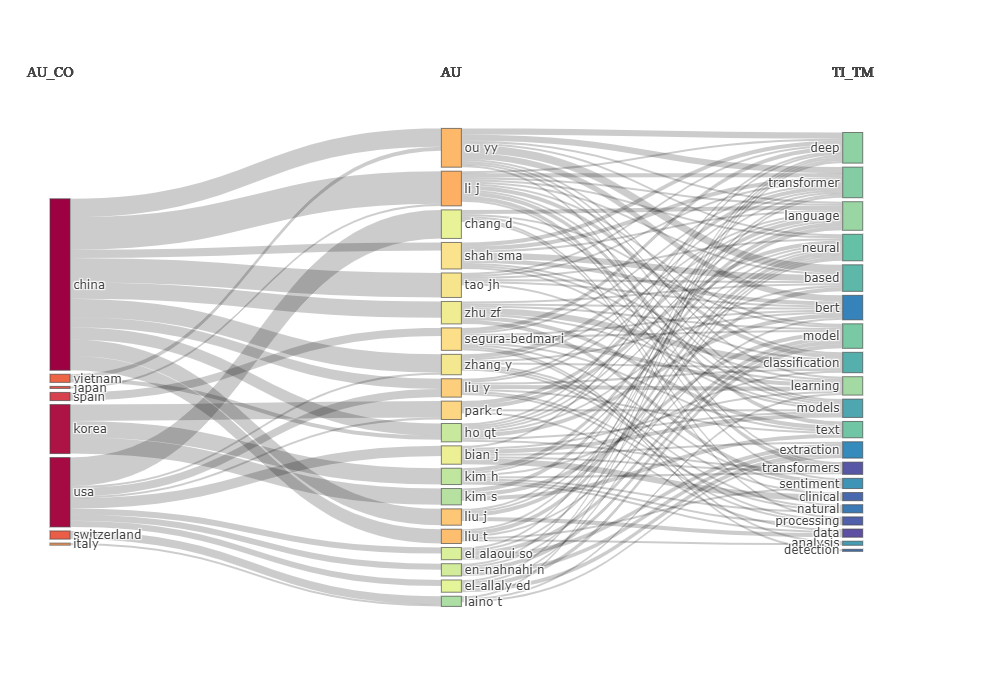
\includegraphics[width=12cm]{experiments/DanielrCardoso/AnaliseBibliometrica/newplot.png}
    \caption{Gráfico de três campos analisando palavras-chave}
    \label{fig:threeDanielrCardoso}
\end{figure}
